\documentclass{beamer}
\usepackage{graphicx}

\title{Deep G-Buffers for stable Global Illumination Approximation}
\author{Ferit Tohidi Far}
\usetheme{Frankfurt}

\begin{document}
	\maketitle

	\begin{frame}
		\frametitle{Content}
		\begin{itemize}
			\item Global illumination
				\begin{itemize}
					\item Pathtracing
					\item Radiosity
				\end{itemize}
			\item Forward rendering
			\item Deferred rendering (with G-Buffers)
			\item Visual effects
				\begin{itemize}
					\item Ambient occlusion
					\item Color bleeding
					\item Soft shadows
					\item Transparency
					\item Reflections
				\end{itemize}
			\item Deferred rendering (with Deep G-Buffers)
		\end{itemize}
	\end{frame}

	\begin{frame}
		\frametitle{Global illumination}
	\end{frame}

	\begin{frame}
		\frametitle{Pathtracing}
	\end{frame}

	\begin{frame}
		\frametitle{Radiosity}
	\end{frame}

	\begin{frame}
		\frametitle{Forward rendering}
	\end{frame}

	\begin{frame}
		\frametitle{Deferred rendering (with G-Buffers)}
	\end{frame}

	\begin{frame}
		\frametitle{Visual effects}
	\end{frame}

	\begin{frame}
		\frametitle{Deferred rendering (with Deep G-Buffers)}
	\end{frame}	

	\begin{frame}
		\frametitle{Results}
		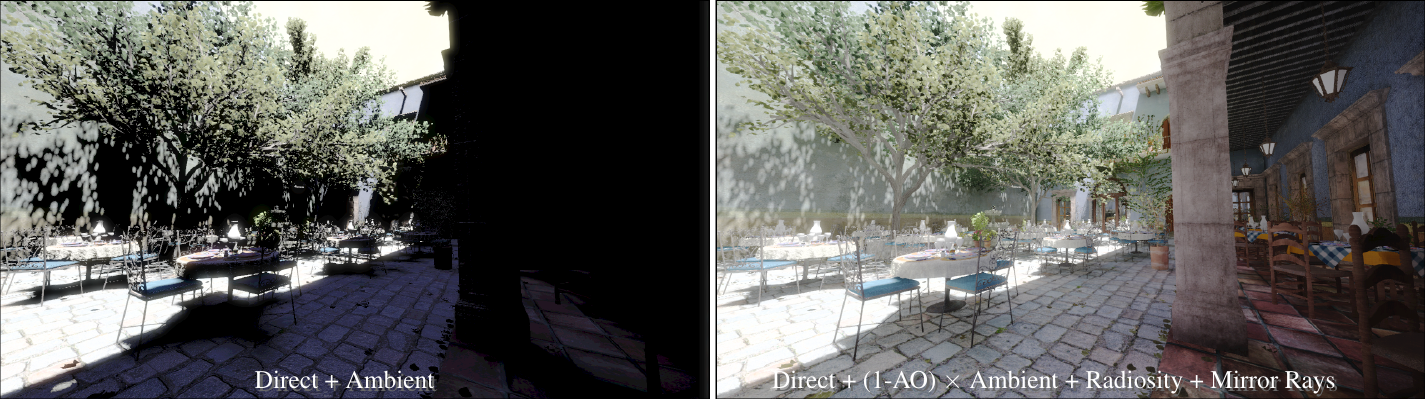
\includegraphics[width=\textwidth]{img/deep_g_buffer_render.png}
		\begin{itemize}
			\item using NVIDIA GeForce 980
			\item image was generated in 10.8ms (92 FPS)
		\end{itemize}
	\end{frame}

\end{document}